%% TeXworks instructions:
% !TeX root = ./report.tex
% !TEX encoding = UTF-8 Unicode
%% !TEX program = arara
%% !TEX TS-program = arara
% !TeX spellcheck = it-IT

% arara: pdflatex: { synctex: yes, action: batchmode, options: "-halt-on-error -file-line-error-style" }
% arara: pdflatex: { synctex: yes, action: nonstopmode, options: "-halt-on-error -file-line-error-style" }

%% Generate a report.xmpdata file with title and authors for PDF/A-compliant format %%
\begin{filecontents*}{\jobname.xmpdata}
    \Title{Maraph1-mp Project Report}
    \Author{Nicholas Brasini\sep Gjulio Jakova\sep Federico Naldini\sep Jacopo Riciputi}
\end{filecontents*}

\documentclass[%
    a4paper,            % specifica il formato A4 (default: letter)
    10pt,               % specifica la dimensione del carattere a 10
    oneside,            % serve per impaginare per stampa solo fronte
    notitlepage         % mette il titolo in una pagina separata (solo per article)
]{article}

\usepackage{a4wide}             % consente di avere più spazio nell'A4

%% ORDINE IMPORTANTE INIZIO %%%%%%%%%%%%
\usepackage[T1]{fontenc}        % serve per impostare la codifica di output del font
\usepackage{textcomp}           % serve per fornire supporto ai Text Companion fonts
\usepackage[utf8]{inputenc}     % serve per impostare la codifica di input del font
\usepackage[
    english,            % utilizza l'inglese come lingua secondaria
    italian             % utilizza l'italiano come lingua primaria
]{babel}                        % serve per scrivere Indice, Capitolo, etc in Italiano

\usepackage{lmodern}            % carica una variante Latin Modern prodotto dal GUST
%% ORDINE IMPORTANTE FINE %%%%%%%%%%%%%%

\usepackage{indentfirst}        % serve per avere l'indentazione nel primo paragrafo
\usepackage{setspace}           % serve a fornire comandi di interlinea standard
\usepackage{xcolor}             % serve per la gestione dei colori nel testo
\usepackage{graphicx}           % serve per includere immagini e grafici

\graphicspath{{./images/}}

\usepackage[%
    strict,             % rende tutti gli warning degli errori
    autostyle,          % imposta lo stile in base al linguaggio specificato in babel
    english=american,   % imposta lo stile per l'inglese
    italian=guillemets  % imposta lo stile per l'italiano
]{csquotes}                     % serve a impostare lo stile delle virgolette

\usepackage{multirow}           % aggiunge la possibilità di raggruppare celle su più righe nelle tabelle

\onehalfspacing%                % Imposta interlinea a 1,5 ed equivale a \linespread{1,5}

\setcounter{secnumdepth}{4}     % Numera fino alla sottosezione nel corpo del testo
\setcounter{tocdepth}{4}        % Numera fino alla sotto-sottosezione nell'indice

\usepackage[%
    depth=3,            % equivale a bookmarksdepth di hyperref
    open=false,         % equivale a bookmarksopen di hyperref
    numbered=true       % equivale a bookmarksnumbered di hyperref
]{bookmark}                     % Gestisce i segnalibri meglio di hyperref
\usepackage{hyperref}           % Gestisce tutte le cose ipertestuali del pdf
\hypersetup{%
    pdfpagemode={UseNone},
    hidelinks,          % nasconde i collegamenti (non vengono quadrettati)
    hypertexnames=false,
    linktoc=all,        % inserisce i link nell'indice
    unicode=true,       % only Latin characters in Acrobat’s bookmarks
    pdftoolbar=false,   % show Acrobat’s toolbar?
    pdfmenubar=false,   % show Acrobat’s menu?
    plainpages=false,
    breaklinks,
    pdfstartview={Fit},
    pdfauthor={Nicholas Brasini, Gjulio Jakova, Federico Naldini, Jacopo Riciputi},
    pdfcreator={Nicholas Brasini, Gjulio Jakova, Federico Naldini, Jacopo Riciputi},
    pdftitle={Maraph1-mp Project Report},
    pdflang={it}
}
\usepackage[utf8]{inputenc} % serve per avere l'indice di tutti i capitoli all'inizio 

%\usepackage[a-1b]{pdfx}
\usepackage[%
    english,italian,    % definizione delle lingue da usare
    nameinlink          % inserisce i link nei riferimenti
]{cleveref}                     % permette di usare riferimenti migliori dei \ref e dei varioref

\title{\LARGE{\textbf{Maraph1-mp Project Report}}}

\author{%
    Nicholas~Brasini\\%
    Gjulio~Jakova\\%
    Federico~Naldini\\%
    Jacopo~Riciputi
}

\date{%
    \small{Paradigmi di Programmazione e Sviluppo}\\%
    \small{Anni accademici 2017--2018 e 2018--2019}
}


\begin{document}
	
    \maketitle
    \clearpage
	\tableofcontents
	\clearpage
    \section*{\Huge {Capitolo 1}\label{chapter1}}
      \section{Processo di sviluppo}\label{sec:process}
        \subsection {Metodologia di sviluppo}\label{subsec:metodology}
        \subsection {Strumenti adottati}\label{subsec:tools}
        
        \clearpage
        
    \section*{\Huge {\textbf Capitolo 2}\label{chapter2}}
    \section{Requisiti}\label{sec:requirements}
         \subsection {Requisiti utente}\label{subsec:requirements:business}
             \subsection {Requisiti funzionali}\label{subsec:requirements:functional}
            \subsubsection[Gioco]{\large {Regole del gioco}\label{subsub:requirements:game}}
            \subsubsection[NoAutenticazion]{\large {Servizio di gioco senza autenticazione}\label{subsub:requirements:noauth}}
            \subsubsection[Autenticazion]{\large {Servizio di gioco con autenticazione}\label{subsub:requirements:auth}}
            \subsubsection[Stanze di gioco]{\large {Servizio delle stanze di gioco}\label{subsub:requirements:lobby}}
            \subsubsection[Interfaccia utente]{\large {Interfaccia grafica per l'utente}\label{subsub:requirements:gui}}
        \subsection {Requisiti non funzionali}\label{subsec:requirements:notFunctional}
        \subsection {Requisiti implementativi}\label{subsec:requirements:implementative}
   
   \clearpage
    \section*{\Huge {\textbf Capitolo 3}\label{chapter3}}
    \section{Design architetturale}\label{sec:design}
       
        
        \subsection[Architettura]{Architettura e pattern utilizzati}\label{subsec:architecture}
         L'architettura del sistema va a basarsi fortemente su un design \textbf{client-server}, all'interno del progetto entrano perciò in gioco due entità fortmente distinte. \\ Per la realizzazione dell'applicazione locale è stato adottato il pattern Model-View-Controller, così da permettere una maggior suddivisione dei compiti, soprattutto per quanto riguarda la parte grafica e logica del gioco dalla sezione d'interazione con il remoto.  \\
        Per il lato server-side invece, dato che le specifiche oltre che a richiedere una parte statica di semplice gestione dati, richiedevano anche una modalità dinamica (real-time), sono stati adottati due differenti pattern.
        \\
        La gestione dei dati è stata affidata a un server che mette a disposizione per i client una serie di chiamate \textbf{API REST}, mentre, per il real-time, la scelta è ricaduta sulla creazione di una sessione di gioco utilizzando il pattern \textbf{Publish-Subscribe}.
        
        
            \subsubsection{Architettura server-side}\label{subsub:architecture:server}
            L'architettura server-side prende spunto, nonostante non la implementi nelle sue piene caratteristiche, da un approccio orientato ai microservizi, così da costruire un modello che sia in un futuro facilmente scalabile. \\
            
            Per fare ciò è stato inserito tra il client e il backend un \textbf{Service discovery}. 
            
            \begin{figure}[h!]
                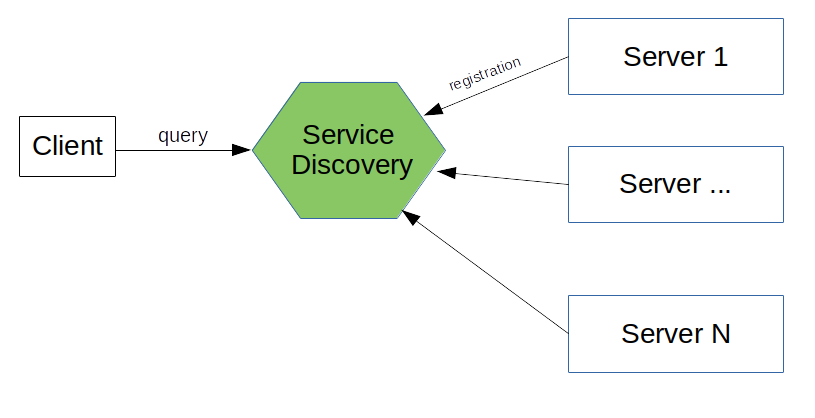
\includegraphics[scale=0.6]{image/ArchitetturaDiscovery.png}
                \caption{Architettura client-server con Service Discovery. Allo start up il server si iscrive sul discovery e viene considerato tra gli endpoint disponibili. A questo punto il discovery lo reputa un componente attivo e vi indirizzerà i client.}
            \end{figure}

            Grazie all'apposizione di un \textit{Service Discovery} tra gli \textit{endpoint} è stata data, a livello di modello, la possibilità all'applicazione di aggiungere servizi e di avere anche più server che si occupano dello stesso, dato che, essendo il \textit{discovery} l'intermediario tra il client e il backend svolge inoltre il ruolo di \textit{Load Balancer}, andando perciò a indirizzare il client verso il servizio con meno carico al momento della chiamata.
            In questo modo l'applicazione risulta, oltre che essere fortemente scalabile, fornire anche \textit{high availability} e una buona tolleranza al fallimento. 
            \\
            Una volta ottenuto un instradamento verso uno dei server disponibili entra in gioco un classico servizio ad API REST che si occupa della gestione dell'utente, sia per la parte social che per la ricerca di una partita. 
            
            A questo punto l'architettura utilizzata cambia. Le richieste del dominio impongono una sessione di gioco attiva capace di mantenere uno stato e le API REST non risultano la miglior soluzione. \\ 
            Per la costruzione di un dialogo in real-time fra tutti i componenti di una partita e il server, che gioca nel ruolo di manager di quest'ultima è stato adottato, come anticipato, il pattern \textbf{Publish-Subscribe}. 
            In questo modo ogni membro della partita in ascolto su di un determinato canale sono capaci di ricevere ed emettere messaggi cosicché, alla produzione di un dato da parte di uno dei partecipanti, tutti gli altri siano pronti a recepirlo e consumarlo per poi eventualmente rispondere tramite una determinata azione.
            
            \begin{figure}[h!]
                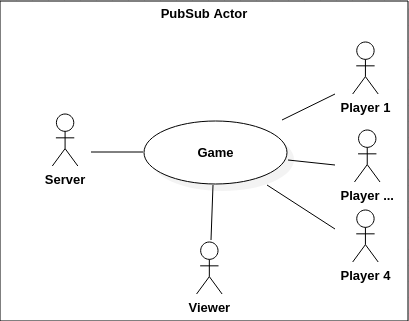
\includegraphics[scale=0.6]{image/PubSubActorDiagram.png}
                \caption{Attori attivi all'interno di un topic del Publish-Subscribe. Il questo caso il topic rappresenta una partita.}
            \end{figure}
            
            \subsubsection{Architettura client-side}\label{subsub:architecture:client}
            Lato client come indicato è stato adottato il pattern MVC. Data la struttura del progetto questa architettura ha permesso uno sviluppo ben distinto delle parti.
            \\
            L'utente infatti, come è possibile vedere dalla figura \ref{fig:UserUseCaseDiagram}, viene indirizzato verso più funzionalità:
            \begin{itemize}
             \item Interfaccia di login o registrazione;
             \item Interfaccia social;
             \item Schermata di gioco.
            \end{itemize}
            Sfruttando i vantaggi del il pattern \textbf{Model-View-Controller} sono stati anche identificati degli attori per la gestione delle parti, così da avere un dialogo tra parte grafica e controller reattiva. 
            La parte di modello invece offre le funzionalità necessarie per gestire al meglio le chiamate al backend per la funzionalità social oltre che per la gestione delle partite vere e proprie.
            
            
	     \begin{figure}[!h]
                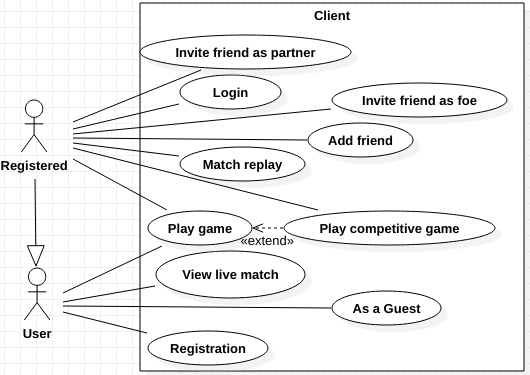
\includegraphics[scale=0.7]{image/UserUseCaseDiagram.png}
                \label{fig:UserUseCaseDiagram}
                \caption{Diagramma dei casi d'uso per le due differenti tipologie d'utente.}
            \end{figure}
            
            


        \subsection{Tecnologie}\label{subsec:technologies}
        Di seguito l'elenco delle tecnologie più rilevanti utilizzate per l'implementazione del progetto.
	  \subsubsection{JavaFX}\label{subsub:tecnologie:javafx}
	    Libreria grafica tra le più importanti nel mondo Java, se non la maggiormente importante. 
	    \\
	    La scelta è ricaduta su di essa in quanto ritenuta più facilmente integrabile con l'idea implementativa. 
	    La dinamicità con il quale è possibile definire file FMXL e la netta suddivisione tra view e controller l'hanno resa per il nostro progetto un'ottima alternativa a Swing.
	    La sezione di JavaFX rappresenta anche l'unica parte scritta in Java, in quanto il framework è stato considerato più maturo rispetto alle librerie disponibili in Scala.
	    
	 \subsubsection{Akka}\label{subsub:tecnologie:akka}
	   Sia lato client che per l'aspetto server è stato utilizzato il framework Akka per la gestione degli attori. 
	   Le capacità di questa libreria di astrarre aspetti complicati di computazione hanno permesso lo sviluppo di un applicazione reattiva su entrambe le parti con il minimo sforzo. 
	   
	 
	 \subsubsection{Akka Cluster}\label{subsub:tecnologie:akkacluster}
	   La realizzazione di un dialogo dinamico tra i client e il server ci ha guidati verso il pattern \textbf{Publish-Subscribe}, per questo motivo la nostra scelta è ricaduta su Akka Cluster. 
	   \\
	   Essendo ben definita un'architettura client-server si è optato per seguire la strada di inglobarla all'interno di un cluster, cosicchè lo scambio di messaggi, tra il client e il server, non avvenga in modalità peer-to-peer.
	   \textbf{Akka Cluster} va inoltre ad aggiungere un'ulteriore scalabilità e affidabilità del sistema dato che, per sua natura, gestisce l'entrata dei nodi nel cluster e i loro ruoli, oltre che a monitorarne le prestazioni e l'eventuale caduta di essi. 
	 \subsubsection{Vert.x}\label{subsub:tecnologie:vert.x}
	  Libreria utilizzata per la gestione del server remoto. Il servizio REST è interamente costruito su Vert.x e lato cliente le stesse chiamate alle API si appoggiano alla parte client della libreria.
	  Tra gli altri si è optato per Vert.x, oltre che per la sua struttura basata sugli eventi asincroni all'interno di un event-loop, per la sua semplicità di deploy. A differenza di altri web server più conosciuti all'interno del mondo Java o Scala come Java EE o Spring, Vert.x è totalmente
	  indipendente e non necessita di un servlet container, permettendo perciò un deploy ancora più immediato.
        \clearpage
    \section{Design di dettaglio}\label{sec:design:details}
    
    \clearpage
    
    \section{Implementazione}\label{sec:implementation}
        \subsection{Nicholas Brasini}\label{subsec:brasini}
        \subsection{Gjulio Jakova}\label{subsec:jakova}
        \subsection{Federico Naldini}\label{subsec:naldini}
        \subsection{Jacopo Riciputi}\label{subsec:riciputi}
	  Lo studente Jacopo Riciputi si è dedicato per la maggior parte del progetto allo sviluppo del servizio di server remoto e gestione dei dati e, in minor entità, di una prima implementazione delle regole di gioco. 
	  \\
	  Nel dettaglio: 
	    \begin{itemize}
	     \item Configurazione di TravisCI;
	     \item Generazione dei Jar;
	     \item Definizione delle regole di gioco;
	     \item Backend;
	     \item Client per richieste HTTP;
	     \item Ricerca di una partita;
	     \item Gestione dei dati.
	    \end{itemize}
	    
	
	\subsubsection{Configurazione di TravisCI}
	  La configurazione di Travis è risulta fin da subito molto semplice, in quanto il servizio è stato utilizzato con l'unico scopo di effettuare i test a ogni push sul repository.
	 
	\subsubsection{Generazione dei Jar} 
	  Per la generazione dei Jar ci si è affidati al plugin \textbf{shadow}. Esso tramite il task \textit{shadowJar}
	  offre la possibilità di generare \textit{fatJar} completi e pronti all'esecuzione semplicemente definendo preventivamente qualche variabile. \\
	  È apparsa qualche difficoltà nel momento in cui si aveva la necessità di generare tre \textit{jar} differenti, uno per ogni \textit{main} presente nel progetto. 
	  Per fare ciò sono stati definiti all'interno del file \textit{build.gradle} tre task, uno per \textit{main}, nei quali viene gestito il tipo \textbf{ShadowJar}, 
	  al quale, per configurazione, definisco un classificatore da associare al jar da creare, la \textit{main class} 
	  e vengono ereditate le dipendenze dal \textit{shadowJar} principale.
	  
	\subsubsection{Definizione delle regole di gioco}
	  Lo scopo iniziale del primo sprint era quello di ottenere una modalità base di gioco nel quale fossero definite le basiche funzionalità di una partita, senza prendere in considerazione l'aspetto distribuito.
	  \\
	  Durante questa sezione mi sono occupato delle sviluppo di una prima versione di quello che poi successivamente è diventato il GameActor, gestore dell'intera partita. 
	  Per fare ciò sono partito subito dalla definizione di un semplice trait che però definisse gli aspetti principali il gioco doveva rispettare. 
	  Il trait in questione è \textbf{Match}.\\
	  Una volta definito, nonostante la sua semplicità, il suo sviluppo ha portato di conseguenza alla definizione di tutti gli aspetti di gioco a esso legati. 
	  Prima di ogni cosa risultava importante definire bene gli interlocutori all'interno della partita, nonostante non se ne conoscesse ancora la sua esatta forma. \\
	  Per questo motivo nasce il trait generico \textbf{BaseTeam}. Esso definisce tutti gli aspetti che un team che prende parte al gioco deve rispettare ma non ne limita la forma, per questo la genericità. \\
	  Una volta definito come fossero gestiti i team e di conseguenza i giocatori che prendevano parte alla partita occorreva iniziare a definire gli aspetti di gioco.\\
	  Per fare ciò ho implementato la classe GameCycle, questo file non fa altro che implementare al suo interno una struttura data simile a una \textit{cyclic queue}. Inizialmente, infatti, mi ero orientato su quest'ultima, ma, non avendo trovato nulla che mi soddisfacesse del tutto si è optato per la costruzione di una classe capace di gestire la situazione creatasi all'interno del progetto. 
	  La classe infatti viene definita fornendole due team e su di essi vi costruisce un una lista di giocatori alternati in base alla suddivisione dei team. Questa lista diventerà poi la base per la gestione dei turni durante la partita. 
	  \\
	  Definiti anche questi aspetti, insieme alle parti sviluppate da Federico Naldini, il quale si è occupato della definizione e gestione del Deck e delle carte, avevo a disposizione tutti gli elementi per completare le regole del gioco. 
	  A questo punto si è semplicemente trattato di definire bene degli stati interni e i metodi per la loro gestione oltre che delineare le regole del gioco.
            \begin{figure}[!h]
                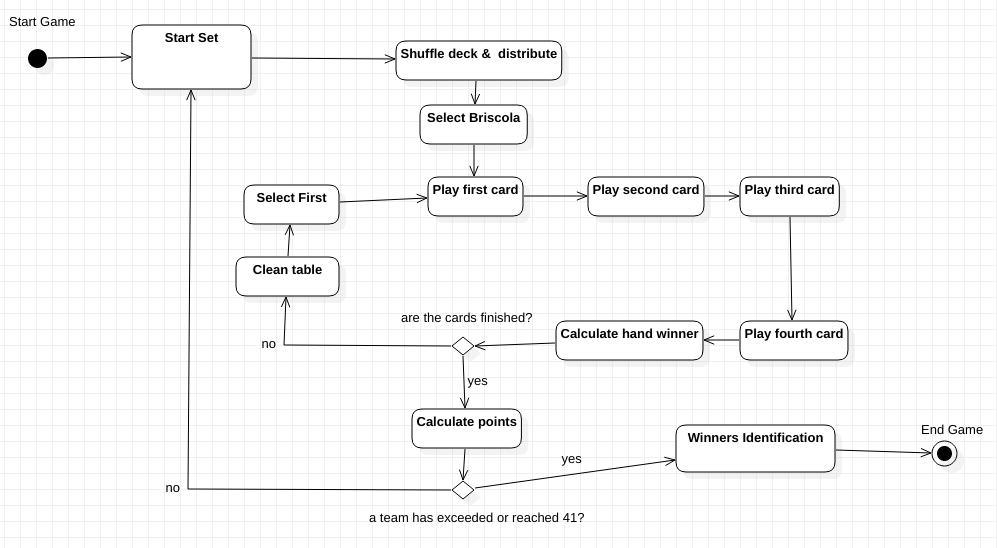
\includegraphics[scale=0.5]{image/MatchStateChar.png}
                \label{fig:MatchStateChar}
                \caption{Diagramma degli stati che analizza i vari stadi di una partita}
            \end{figure}
	  \\
	  \subsubsection{Backend}
	  La parte server è stata costruita sopra al framework Vert.x. Questa libreria è stata prediletta sopra altre per la sua semplicità, soprattutto di deploy. Rispetto ad altre risultava però leggermente acerba e da essa non riuscivamo a ottenere esattamente tutto ciò che desideravamo. 
	  \\
	  Per un lato server ben ingegnerizzato e facilmente scalabile si è incappati quindi nella necessità d'inglobare gli elementi offerti da Vert.x in classi più ad alto livello, che permettessero al programmatore di evitare il contatto tutte le volte con gli aspetti base della libreria. 
	  In questo senso si è intervenuti principalmente tramite le classi \textbf{Router}, \textbf{RouterResponse} e \textbf{Dispatcher}.
	  
	  Il file \textbf{Router} funge da \textbf{Adapter} della classica gestione degli handler in Vert.x.\\\
	  All'interno di esso viene definito il trait \textbf{Request} il quale si occupa d'inglobare aspetti di Vert.x per la gestione delle richieste così da poter rendere generica la definizione di una richiesta.
	  A estendere questo trait vi sono le \textit{case class}, implementate basandosi sul pattern \textbf{strategy}, \textbf{GET} e \textbf{POST}. Queste non fanno altro che definire internamente il metodo HTTP al quale risponderanno e prendere in ingresso il \textbf{Vert.x.Router} sul quale il server è in ascolto, il \textit{path} sul quale la richiesta sarà resa disponibile e un \textit{handler}, nel quale, la richiesta, dopo essere stata gestita dovrà rispondere al chiamante. \\
	  La funzione che andrà a gestire la richiesta avrà disponibile, come parametro, due elementi, un \textit{RoutingContext}, classe definita da Vert.x, che mette a disposizione all'\textbf{handler} tutti i dati inerenti alla richiesta e un \textbf{RouterResponse}.
	  Quest'ultima è la seconda delle tre classi create per l'ottimizzazione dell struttura creata. 
	  \\
	  \textbf{RouterResponse} funge da \textit{wrapper} della classe \textit{RoutingContext} fornendo all'\textit{handler} metodi semplici per rispondere alla richiesta. Definisce infatti il metodo \textit{sendResponse()}, il quale, dato in ingresso un JsonResponse, si occupa di serializzare il parametro in una stringa JSON e d'inviarla al \textit{client}. 
	  \\
	  A livello di progettazione inoltre è stato definito che venissero considerate come positive solamente le risposte con il codice 200 come status nell'\textit{header}. La semplice chiamata di questo metodo risponderà inserendo questo codice nel messaggio, diversamente, chiamando precedentemente \textit{setError} si può definire un differente codice oppure tramite la \textit{setGenericError} si produrrà una risposta con lo status d'errore di default 409.
	  Come precedentemente indicato, per completare la richiesta è necessario fornirle un \textbf{JsonResponse}. Questo trait non fa altro che definire un tipo di classe che ha lo scopo di essere serializzata e deserializzata tramite la libreria \textbf{json4p} in stringhe JSON. \\
	  A fungere, infine, da collante tra queste parti di modello vi è il \textbf{Dispatcher}, al suo interno infatti vengono associati alle richieste gestite dal server i rispettivi \textbf{handler}, per poi terminare con il \textit{deploy} del backend.
      
	\subsubsection{Client per richieste HTTP}
	  Il client HTTP costruito sulla libreria \textbf{Vert.x Web-client} si struttura similarmente alla classe Router. Definisce infatti un trait che stabilisce tutti gli elementi necessari per portare a termine una richiesta. 
	  A implementare il trait vi sono le classi GetRequest e PostRequest. Queste differiscono non solo nel metodo HTTP della chiamata ma anche nella gestione dei parametri. Entrambe, infatti, prendono in ingresso una mappa di parametri, ma, mentre la prima li serializza all'interno dell'url, le chiamate post effettuano l'invio dei parametri come \textit{form-body}.\\
	  A completare la classe vi sono i due \textbf{handler}, \textbf{onSuccess} oppure \textbf{onFail}. Il primo verrà richiamato solamente nel caso in cui la chiamata ha esito positivo e il suo \textit{status code} è 200. \\
	  Il secondo invece, per esclusione, viene notificato in ogni caso d'errore, sia che la chiamata lanci un'eccezione sia che la chiamata venga effettuata ma ottenga una risposta con un codice di errore. In questo caso viene fornita all'\textit{handler} un'eccezione creata appositamente con il messaggio d'errore ottenuto dalla risposta. 
	  
        \subsubsection{Ricerca di una partita}
          Il server mettette a disposizione dei client un'apposita API REST per la ricerca di una partita. L'API accetta come parametri fino a quattro giocatori e restituisce al chiamante l'id della partita a cui è stato assegnato.
          \\
          Una volta ricevuta la richiesta, il server, risveglia un apposito attore, il \textbf{LobbyActor} che ha il compito specifico di, in base al tipo di partita, classificata o meno, ricercare una lobby disponibile per i giocatori nella richiesta. Al suo interno il \textit{LobbyActor} ricerca ricorsivamente una lobby che rispetti i team definiti dalla richiesta, nel caso in cui questa non esiste, crea genera una, alla quale associa i componenti delle squadre. Dopo di che, in entrambi i casi risponde inserendo l'id della partita nel corpo del messaggio ed esegue un controllo. Il controllo in questione verifica se la lobby risulta essere composta da quattro giocatori. Se il controllo ha esito positivo crea un nuovo \textbf{GameActor},
        
        \subsubsection{Gestione dei dati}
          A supporto della parte server del progetto era necessario inserire un database per il salvataggio dei dati dell'utente, le relazioni social, e le partite. 
          \\
          La scelta è ricaduta su \textbf{Redis}, database \textit{in-memory} particolarmente performante, anche se, si è optato per questa soluzione data la semplicità con il quale è possibile modellare i dati al suo interno.
          \\
          La progettazione di questa sezione è stata però pensata per essere indipendente dal database scelto. È possibile infatti trovate tre trait generici: \textbf{DatabaseInterface}, \textbf{GameDatabaseInterface}, \textbf{UserDatabaseInterface} i quali definisco i metodi che il \textit{DAO} deve fornire ma non ne specifica alcuna caratteristica. Questo semplificherebbe un eventuale futuro cambiamento del motore di database. \\
          In questa parte di sviluppo dell'accesso ai dati è stata sfruttata, ancora più che nelle altre mie parti del progetto, la programmazione funzionale nell'ottica di creare un passaggio d'informazioni tramite \textit{callback}. Uno stile di programmazione di questo tipo però rischiava di portare a una bassa qualità di codice. Aiutandosi però con i metodi offerti dalla classe \textbf{Future}, si è mantenuto il codice il più possibile appiattito, senza ricadere in eventuali \textit{pyramid of doom}.
          \\
          A estendere questi \textit{trait} vi sono le classi: \textbf{RedisUtils}, \textbf{RedisGame}, \textbf{RedisUser}, queste implementano i metodi definiti nelle rispettive interfacce eseguendo, in base alle esigenze, le apposite query su \textbf{Redis}.
          \\
          Per quanto riguarda l'esecuzione di comandi sul database, inizialmente, vi era una continua ripetizione di codice, data la necessità a ogni interazione di:
          
          \begin{enumerate}
           \item Ottenere la connessione con il database;
           \item Eseguire una o più query;
           \item Chiudere la connessione se non più utilizzata.
          \end{enumerate}
          
          Per evitare tutto questo, dato che poteva portare anche facilmente all'errore, sono nate le classi \textbf{Query} e \textbf{BlockingQuery}. Queste hanno esattamente lo stesso funzionamento, si differenziano solamente per il \textit{client} usato per eseguire i comandi, nel primo caso si tratta di \textbf{Rediscala}, libreria scala reattiva e non bloccante, mentre nel secondo di \textbf{Jedis}, principale \textit{client} Redis per Java che però non sfrutta per il meccanismo delle \textit{Future}. 
          \\
          Proprio ispirandosi a quest'ultime nascono le due classi sopraccitate. \\
          \textbf{Query} e \textbf{BlockingQuery} non fanno altro che offrire uno \textit{spazio} delineato per eseguire i comandi. Prendono infatti in ingresso un \textit{body}, che non è altro che una funzione alla quale è offerta come parametro una connessione aperta con il database. Terminato il \textbf{body} queste classi offrono anche la possibilità di definire una \textit{callback} per ottenerne il valore di ritorno ed eseguire eventuali altre operazioni.
          Al termine del suo utilizzo la connesisone verrà poi automaticamente chiusa, tramite il metodo comune \textit{closeConnection()}, implementato per entrambe le classi per facilitarne la chiusura.
          La funzione è stata definita tramite il costrutto \textbf{Pimp-my-Library}, pattern che, con il senno di poi, mi sono pentito di non aver utilizzato più spesso all'interno del progetto, perché personalmente ritenuto decisamente efficiente e dalle tante potenzialità.
          
          
          

          
          
          
      
      \clearpage
      
        
    \section{Retrospettiva}\label{sec:retrospective}

\end{document}
